\TODO{rethink about this chapter}

The exploration of space has witnessed a surge in intensity, with an increasing number of countries aspiring to venture into this domain. Noteworthy examples include NASA's initiation of the Artemis mission, which aims to return to the Moon by 2024. Similarly, China has unveiled its plans to establish a lunar base on the lunar surface by the 2030s, while the European Space Agency (ESA) has also embarked on a lunar lander mission. Most recently, a Japanese lunar lander mission was launched; however, it regrettably encountered failure.

Under these circumstances, the study of solar energetic particles (SEPs) assumes greater significance. SEPs pose a significant radiation hazard for future human exploration on the lunar surface. The most hazardous SEP events have the potential to induce radiation increases of substantial magnitude.

The Chang'E-4 mission, initiated in 2019, coincided with a period of solar minimum characterized by a scarcity of SEP events. However, as solar activity has intensified, a growing number of SEP events, including prolonged-duration and high-intensity SEPs, have been observed to reach the lunar surface and have been detected by the Lunar Neutron and Dosimetry (LND) instrument. For example, Guo et al. (2023) recently reported the first Ground-Level Enhancement (GLE) events of Solar Cycle 25, which were concurrently detected by instruments deployed on the Moon, Earth, and Mars. It is noteworthy that the LND instrument primarily captured the decay phase of these events.

In the concluding sections of this thesis, a comprehensive list of SEP events detected by the LND instrument on the lunar far-side surface between 2019 and 2023 is provided, further contributing to our understanding of these phenomena.

%For sure LND is outside of the mangetosphere, but still that is one of the thing worth to look at. How the SEP propogarting across the magnetosphere and arrive the magnetosphere tails.

In this chapter, we present a comprehensive study of the initial solar energetic particle (SEP) event detected by the Lunar Neutron and Dosimetry (LND) instrument in May 2019, which occurred during the first half-year of the Chang'e-4 mission. This SEP event is associated with an M-class flare originating from solar active region (AR12470) located on the eastern hemisphere, more than 110 degrees away from the Earth's magnetic footpoint on the solar surface. Observations conducted by the Solar and Heliospheric Observatory/Large Angle and Spectrometric Coronagraph (SOHO/LASCO) and Solar Terrestrial Relations Observatory (STEREO) revealed the presence of a slow, narrow, and westward moving coronal mass ejection (CME).

The primary objective of this study is to utilize the first SEP event observed by LND to validate the data products produced during SEP occurrences and assess the instrument's performance under such conditions. By cross-calibrated the proton measurements between LND and other already existed particle instruments at L1 point, specifically the EPHIN onboard SOHO and ACE/EPAM, we found that the LND provide reliable charged particle measurement, both on time and flux level.

Additionally, we aim to investigate its extensive spatial distribution, and discuss the particle propagation mechanisms involved in its traversal across considerable distances between the active region and the Earth's magnetic footpoint. 
The following article is reproduced from \textcite{Xu2020ApJ} by permission of the AAS:\\

\noindent\pubcite{Xu2020ApJ}\\
\strut\hfill Own contribution: 80\%

\newpage
\newcounter{includepdfpageAPJLTwenty}

\addtocounter{section}{1}
\setcounter{section}{1} 
% \phantomsection
% \addcontentsline{toc}{section}{\arabic{chapter}.\arabic{section} First Solar Energetic Particles Measured on the Lunar Far-side(Publication ApJ Letter 2020)}
%
\phantomsection
\addcontentsline{toc}{section}{\arabic{chapter}.\arabic{section} Introduction}
\label{sec:paper_xu2020}
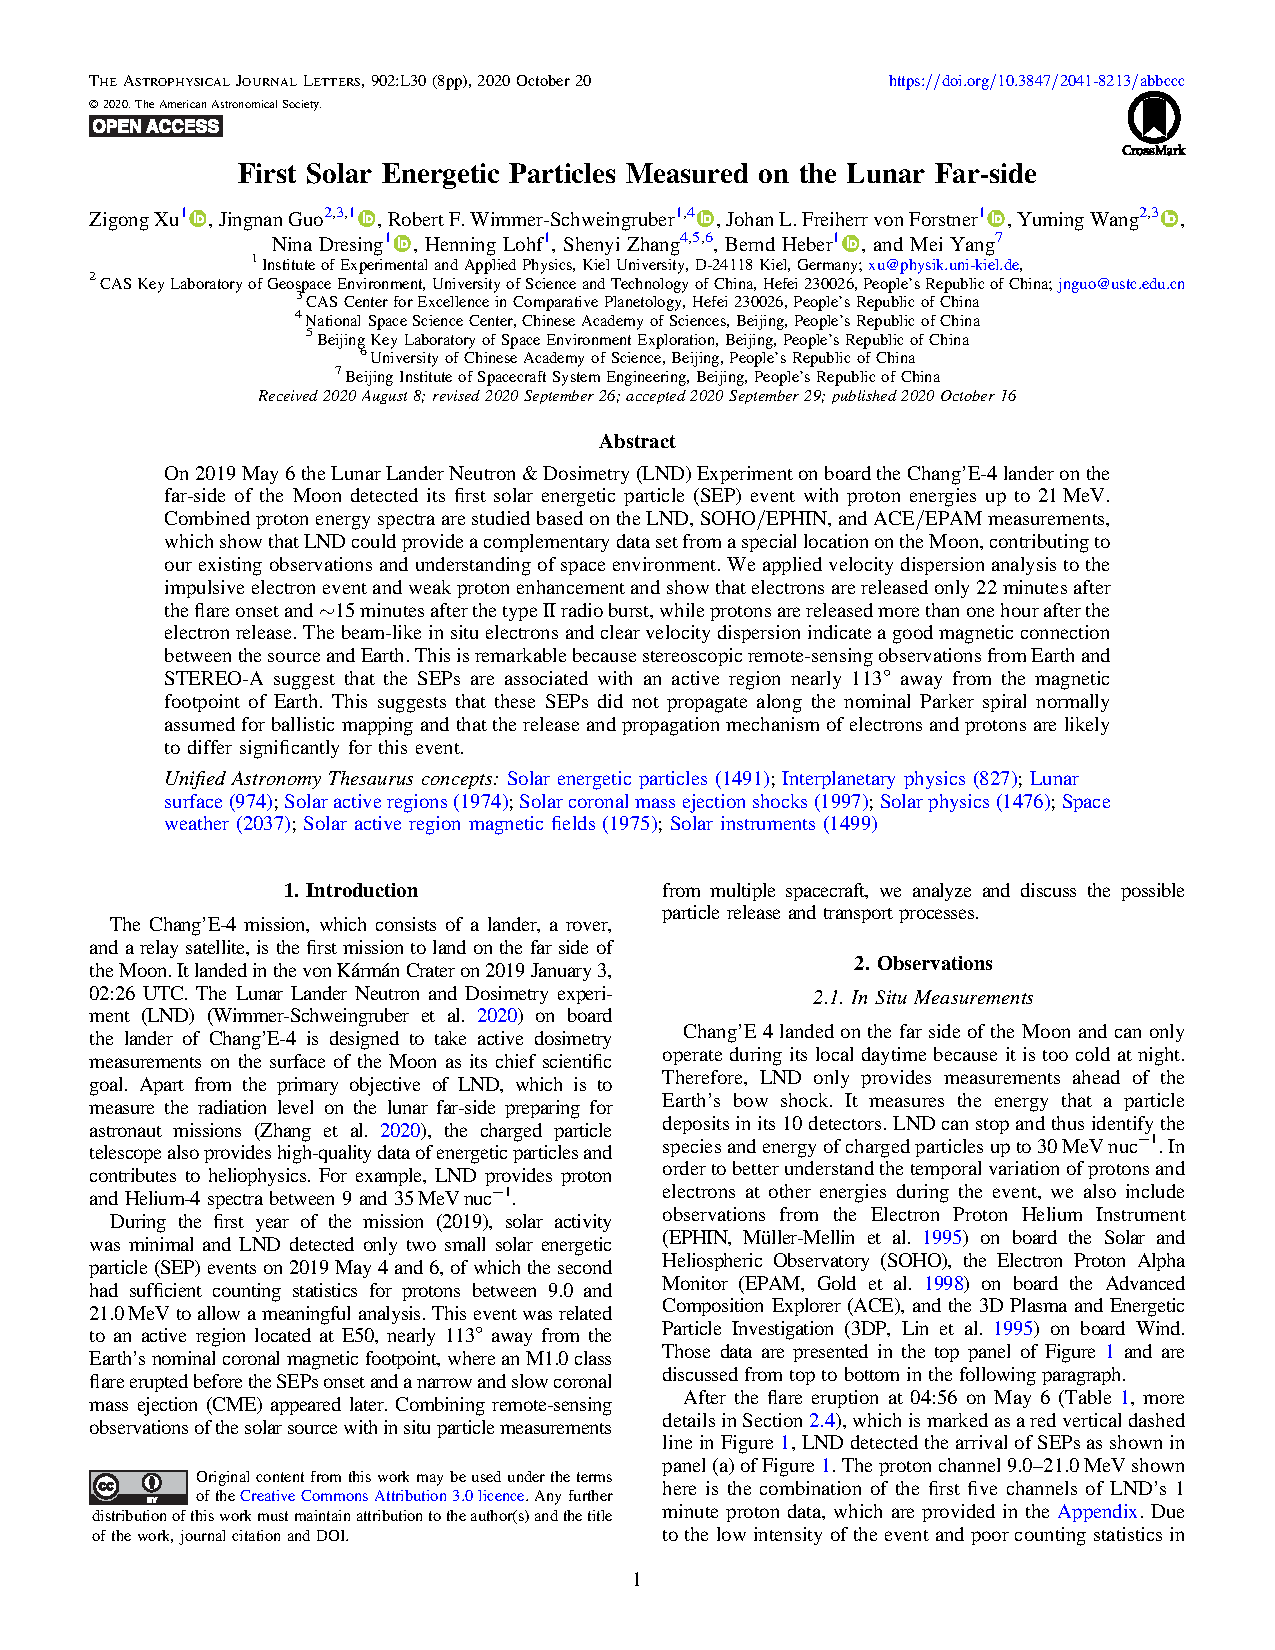
\includepdf[pages={1}, link, linkname=paper_xu2020, scale=.9, pagecommand={\refstepcounter{includepdfpageAPJLTwenty}\label{paper_xu2020.\theincludepdfpageAPJLTwenty}}]{publications/Xu_et_al_2020_ApJL.pdf}
%
\addtocounter{section}{1} 
\phantomsection
\addcontentsline{toc}{section}{\arabic{chapter}.\arabic{section} Observations}
\includepdf[pages={2-4}, link, linkname=paper_xu2020, scale=.9, pagecommand={\refstepcounter{includepdfpageAPJLTwenty}\label{paper_xu2020.\theincludepdfpageAPJLTwenty}}]{publications/Xu_et_al_2020_ApJL.pdf}
%
\addtocounter{section}{1} 
\phantomsection
\addcontentsline{toc}{section}{\arabic{chapter}.\arabic{section} Summary and Discussion}
\includepdf[pages={5-6}, link, linkname=paper_xu2020, scale=.9, pagecommand={\refstepcounter{includepdfpageAPJLTwenty}\label{paper_xu2020.\theincludepdfpageAPJLTwenty}}]{publications/Xu_et_al_2020_ApJL.pdf}
%
\addtocounter{section}{1} 
\phantomsection
\addcontentsline{toc}{section}{\arabic{chapter}.\arabic{section} Appendix}
\includepdf[pages={7}, link, linkname=paper_xu2020, scale=.9, pagecommand={\refstepcounter{includepdfpageAPJLTwenty}\label{paper_xu2020.\theincludepdfpageAPJLTwenty}}]{publications/Xu_et_al_2020_ApJL.pdf}
%
\addtocounter{section}{1} 
\phantomsection
\addcontentsline{toc}{section}{\arabic{chapter}.\arabic{section} References}
\includepdf[pages={8}, link, linkname=paper_xu2020, scale=.9, pagecommand={\refstepcounter{includepdfpageAPJLTwenty}\label{paper_xu2020.\theincludepdfpageAPJLTwenty}}]{publications/Xu_et_al_2020_ApJL.pdf}
